
\subsection{Achieving the goal: less waiting time}

Since the main goal of this assignment is speed, the design is focused on minimizing waiting time (stalling). The two most successful approaches we tried are the following:\\

\subsection{Approach 1: Co-P on the BUS}

Following the assignment description, we applied a specially engineered Co-P which can be interacted with through the BUS, as seen in figure \ref{fig:designBus1}. This design makes it possible to do the required calculations, and then store the 32 previous data points in local registers. This is less time consuming, since by not saving and loading from a circular array\footnote{The circular array, is a concept described in assignment 2. Enabling easy access to 32 values in an array with a sweeping index.} in the randomly accessible memory (RAM). \\ 

\begin{figure}[H]
    \centering
    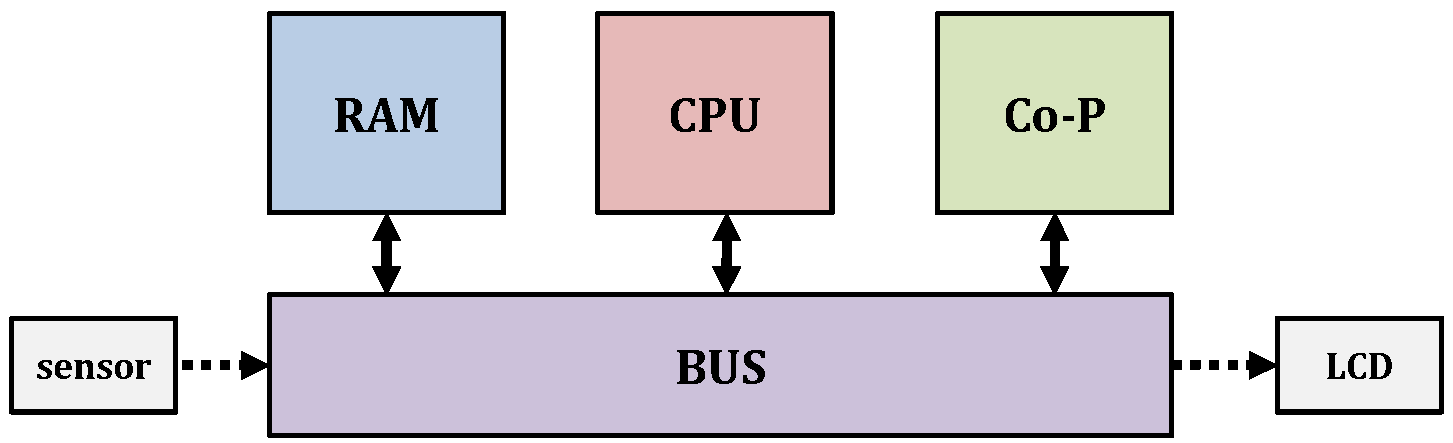
\includegraphics[width=0.8\textwidth]{1Design/fig/designBus1.pdf}
    \caption{In approach 1, all communication between components happens through the bus.}
    \label{fig:designBus1}
\end{figure}

This design supposedly lowers the amount of BUS time, and calculation time. The main CPU is used only for sending information between RAM\footnote{In this case, the RAM is simulating data from the sensor, and the data output to the LCD.} and the Co-P. This makes it possible to strip the CPU of all unused components, minimizing area and thereby energy usage, if necessary. Since the Co-P is specifically made to implement the MWI filter (like the processor in A2), the resources required is also kept at a minimum. 

\subsection{Approach 2: Co-P linked directly to CPU}

This design is a more direct approach to parallelize the communication with the BUS, and the computation involved with applying the filter. Since the main issue is waiting for the BUS to load/store data points, this design focuses on computing the MWI filter, while the main CPU is waiting for the BUS, as seen on figure \ref{fig:designBus2}. \\

In order to achieve this parallelization, we considered two options: Either change the BUS system, making it possible to have two BUSes active at the same time, or to link the CPU directly to the Co-P. We chose the latter as it is both easier to implement, and probably more energy efficient.

\begin{figure}[H]
    \centering
    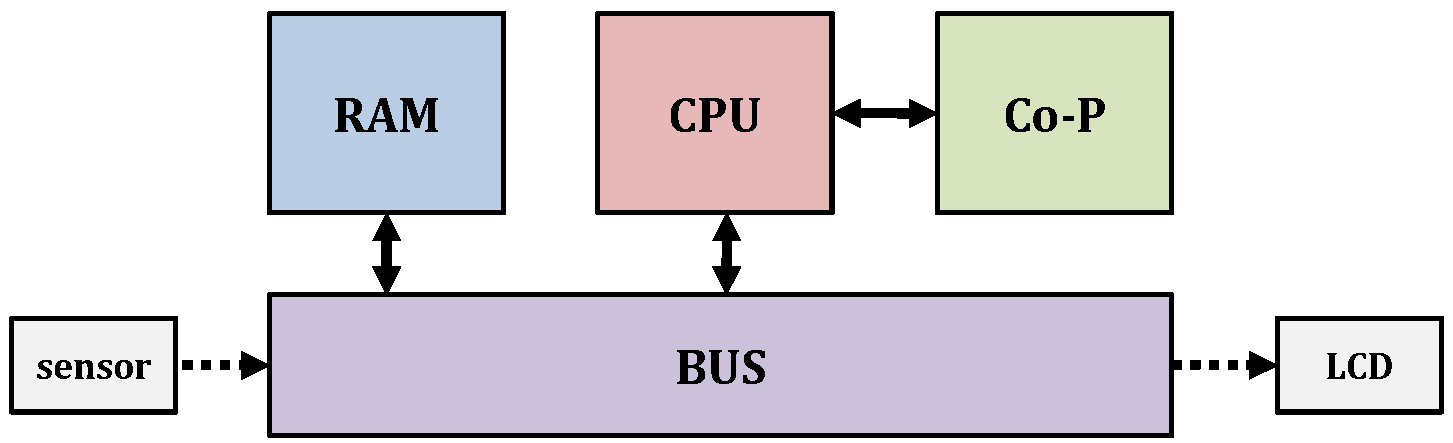
\includegraphics[width=0.8\textwidth]{1Design/fig/designBus2.pdf}
    \caption{In approach 2, Communication between CPU and external memory happens through the bus. Communication between CPU and Co-P happens through a direct connection.}
    \label{fig:designBus2}
\end{figure}

By linking the Co-P to the main CPU directly, the two processors can swap values directly through a handshake. This also implies that the two processors do not need the same clock period. CPU is still in charge of data transfer, so it remains the central processor (as implied by the name \underline{C}entral \underline{P}rocessing \underline{U}nit).

\subsection{Structural vs. behavioral design}\label{sec:structuralOrBehavioralDesign}

Structural designs are closer to the real hardware design, since the actual components and signals are set, representing real chips and wires. Behavioral designs are more applicable for abstract designs, since it allows more complex functionality. By being more abstract, behavioral designs must be interpreted before implemented in hardware and fabricated.\\

We wanted experience in both structural and behavioral design. In assignment 2, we successfully designed and implemented a customized processor structurally. In assignment 3, therefore, we chose to design and implement the Co-P behaviorally. \\

While the Co-P is designed and implemented behaviorally, The CPU is kept structural, as it is the processor from assignment 2, re-purposed to control communication with the Co-P and external memory.

\subsection{Controlling the Co-P}

The two designs are controlled differently. \\

\textbf{Design 1:} using the BUS, Co-P communicates through a \texttt{slavebusinterface}, the same way as the \texttt{DataMem} and the \texttt{Sensor}\footnote{See given template: Platform.fdl.}. This utilizes handshakes and acknowledges already implemented in the BUS. This also means that the BUS must wait for the Co-P to calculate the MWI filter, before it can return the filtered value to the CPU. \\

\textbf{Design 2:} Co-P and CPU are directly linked, so both processors do an internal handshake through a 1 bit flag. Once both processors are ready to do the data transfer, and both processors anticipate the transaction, they interact. When not interacting, the processors either work independently, or in the case of one processor anticipating a handshake, it waits for the other processor to reciprocate the handshake. This ensures that data transfer only occurs when both processors are ready. \\


\subsection{Changes to the CPU from A2}
Energy is used when bits flip, so high activity implies high energy use, but unused components (leftover area) does not necessarily imply high energy use. Hence removing functionality from the CPU when "converting it" to a Co-P is not a high priority. Since the CPU in A2 was already optimized for applying the filter and communicating with the external memory, not much has changed. \\

\textbf{FLTR (initiate filtering):} In design 1, the CPU has an extra instruction (\texttt{FLTR}, apply the \underline{f}i\underline{lt}e\underline{r}). The \texttt{FLTR} instruction sends the BUS to Co-P with data. This is accomplished by \texttt{FLTR} altering \texttt{M\_cmd}, specifically the destination segment: from slave 2 (external memory) to slave 4 (CO-P).\\

\textbf{COPR (swap data with Co-P):} In design 2, the CPU has an extra instruction (\texttt{COPR}, interacting with \underline{co}-\underline{pr}ocessor), for swapping data with the Co-P. The data swap requires that both processors anticipate the handshake. The signal for the handshake is controlled by the processors respective \texttt{CONTROL}s, and the data is transferred through the their \texttt{SHUTTLE} components. This way, the CPU utilizes the stall implementation in \texttt{SHUTTLE} from assignment 2. \\

